\documentclass{standalone}
\usepackage{tikz}
\usepackage{ctex,siunitx}
\setCJKmainfont{Noto Serif CJK SC}
\usepackage{tkz-euclide}
\usepackage{amsmath}
\usetikzlibrary{patterns, calc}
\usetikzlibrary {decorations.pathmorphing, decorations.pathreplacing, decorations.shapes,}

\begin{document}
\small
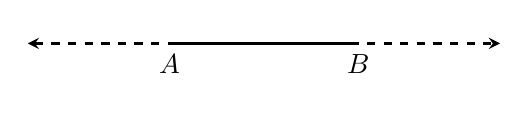
\begin{tikzpicture}[>=stealth,scale=1]
  \tkzSetUpPoint[fill=black]
  \useasboundingbox(-3,0.2)rectangle(3,-0.6);
  \draw[<->, dashed, thick](-3,0)--(3,0);
  \draw[very thick](-1.2,0)node[below]{$A$}--(1.2,0)node[below]{$B$};
\end{tikzpicture}
\end{document}